\section{Introduction to the Problem}
Listing problems are common problems in cambinatorics. In general, listing problems 
focus on enumerating the objects of a given finite set in some specific order. The listing problem in this thesis 
will be termed \emph{The Canonical Ladder Listing Problem}. The problem is stated as follows: Let $\pi_{N}$ be one of $N!$ arbitrary permutation of $[1 \dots N]$. 
Let \emph{The Canonical Ladder} be a unique ladder from $OptL\{\pi_{N}\}$. Let $CanL{\pi_{N}}$ be the set of all canonical ladders for 
all $N!$ permutations of order $N$. Let $L_{i}$ be the canonical ladder of some arbitrary permuation $OptL\{\pi_{N_{i}}\}$. A \emph{change} is defined as the insertion or 
deletion of one or more bar(s) to get from $L_{i}$ to $L{i+1}$, or the relocation of one or more bars in $L_{i}$ to get to $L_{i+1}$. The relocation of a bar 
is defined as moving a bar from a given row and column, to a new row and column in the ladder. The \emph{Listing Problem} asks given all permutations of 
order $N$, is there a way to generate the canonical ladder from each $OptL\{\pi_{N}\}$. 
Furthermore, if there is a way to do so, what is the most efficient way to do so. Efficiency is defined as 
using minimal change to transition from $L_{i}$ to $L_{i+1}$. For example, let $N=4$, there are $N!$ or 24 permutations 
of order $N$. $|CanL{\pi_{N}}=24|$; therefore there are 24 canonical ladders, one from each $OptL\{\pi_{4}\}$. Is there a way to generate 
all 24 canonical ladders for each $OptL\{\pi_{N}\}$? Furthermore, if there is such a way, what is the most efficient way 
to do so; i.e. the algorithm that requires the minimal amount of change to get from $L_{i}$ to $L_{i+1}$. See Table -- for 
the 24 permutations of order 4.
\begin{table}[]
    \begin{center}
       \begin{tabular}{|c |c |c |c |}
        \hline
        1234 & 1243 & 1324 & 1342 \\ \hline
        1423 & 1432 & 2143 & 2134 \\ \hline 
        2314 & 2341 & 2413 & 2431 \\ \hline 
        3124 & 3142 & 3214 & 3241 \\ \hline 
        3412 & 3421 & 4123 & 4132 \\ \hline 
        4213 & 4231 & 4312 & 4321 \\ \hline 
        
    \end{tabular}
    \caption{Table for all 4!, 24, permutations of order 4} 
    \end{center}

 \end{table}



Each of these permutations has one or more ladders in each of their respective 
$OptL\{\pi\}$. The canonical ladder listing  problem asks, given some arbitrary $N \geq 1$,
what is the most efficient way to list $CanL\{\pi_{N}\}$. Recall that in order to get from $L_{i}$ to $L_{i+1}$, at least one of the 
two changes must be applied to $L_{i}$ to get to $L_{i+1}$. At least one bar has to be removed/added or at least one bar 
has to be reolocated in $L_{i}$ to get to $L_{i+1}$.

\begin{theorem}
    In order to transition from canonical ladder $L_{i}$ to canonical ladder $L_{i+1}$, at least one bar has to be added or 
    removed from $L_{i}$ or at least one bar has to be relocated in $L_{i}$.
\end{theorem}
\begin{proof}
    We begin this proof by contradiction. Suppose $L_{i}$ is some arbitrary canonical ladder for permutation of 
    order $N$. Suppose that $L_{i+1}$ is the next canonical ladder in the set of canonical ladders. Each canonical 
    ladder represents a network of adjacent transposisitions of the corresponding permutations, $\pi_{i}$ and 
    $\pi_{i+1}$ used to sort $\pi_{i}$ and $\pi_{i+1}$ respectively. $\pi_{i}$ and $\pi_{i+1}$ are unique. Let $Inv{\pi}$ 
    be the set of all inversions is $\pi$. Let $AdjInv{\pi} \subset Inv{\pi}$ be a subset of inversions in $\pi$
    that are adjacent. A bar in $L_{i}$ and $L_{i+1}$ uninverts an adjacent inversion in from $AdjInv{\pi_{i}}$ and $AdjInv{\pi_{i+1}}$ respectively. 
    Note, that when an adjacent inversion is uninverted, a new intermediate permuation is derived from $\pi$. Let $IntPi(\pi)$
    be the permutation of intermediate permutations, beginning with $\pi$ that result from performing adjacent transpositions on $AdjInv{\pi}$, terminating with 
    the sorted permutation. The row in the ladder represents the order of uninverting adjacent transpositions in some intermediate permutation in $IntPi(\pi)$.
    For example, row 1 in $L_{i}$ represents uninverting adjacent inversions in $\pi_{i}$. The result of uninverting these 
    adjacent inversions is the second intermediate permutation in $IntPi(\pi)$, $\pi'$. Row two represents uninverting the adjecent 
    inversions in $\pi'$ resulting in $\pi''$, etc. If no bars are added or removed from $L_{i}$ then 
    the number of bars in $L_{i+1}$ is the same as in $L_{i}$. This means that the number of adjacent inversions that are uninverted 
    in $\pi_{i}$ is the same as in $\pi_{i+1}$. Next, suppose that no bars are relocated in $L_{i}$ to get to $L_{i+1}$. This would 
    mean that the same adjacent inversions in $\pi_{i}$ exist in $\pi_{i+1}$ and furthermore, the order in which these adjacent 
    iversions were uninverted would be the same for $\pi_{i}$ and $\pi_{i+1}$; in other words the $IntPi(\pi_{i})=IntPi(\pi_{i+1})$ But this is a contradiction, 
    seeing as $pi_{i}$ and $pi_{i+1}$ are unique. Therefore, at least one 
    bar has to be added or removed from $L_{i}$ to get to $L_{i+1}$ or at least one bar in $L_{i}$ has to be relocated to get to $L_{i+1}$.
    See fig- for an example of $L_{3 1 4 2}$ with the corresponding $IntPi(3 1 4 2)$.
\end{proof}

\begin{figure}[!htp]
    \begin{center}
    \begin{tikzpicture}
        %%draw the lines
        \draw(0, 0) to (0, 4);
            \node at(0, 4.3){3};
            \node at(0, -0.3){1};
        \draw(2, 0) to (2, 4);
            \node at(2, 4.3){1};
            \node at(2, -0.3){2};
        \draw(4, 0) to (4,4);
            \node at(4, 4.3){4};
            \node at(4, -0.3){3};
        \draw(6, 0) to (6, 4);
            \node at(6, 4.3){2};
            \node at(6, -0.3){4};
        \node at(8, 3){3,1,4,2};
        \node at(8, 2){1,3,2,4};
        

        \node at(-2, 4.3){$R_{0}$};
        \node at(-2, 3){$R_{1}$};
        \node at(-2, 2){$R_{2}$};
        \node at(-2, -0.3){$R_{3}$};

        %%draw the bars
        \draw(0, 3) to (2, 3);
        \draw(2, 2) to (4, 2);
        \draw(4, 3) to (6,3);

    \end{tikzpicture}
    \end{center}
    \caption{The rows are on the left of the ladder designating the order in which the adjacent inversions will be uninverted.
    On the right is the $IntPi(3,1,4,2)$ that results from the ladder univerting  the adjacent inversions in 3,1,4,2 in the order 
    of the rows. $IntPi(3,1,4,2)=((3,1,4,2), (1,3,2,4), (1,2,3,4))$}
\end{figure}

In this thesis, two listing algorithms were used to generate the canonical 
ladders for each $OptL\{\pi_{N}\}$. The first of these listing algorithms 
is a modification of the Steinhaus-Johnson-Trotter permutation listing algorithm. 
The second listing algorithm is, as far as I know, a novel algorithm. 
It is termed the cyclic-inversion algorithm. Both of these algorithms will 
be described, explained and analyzed throughout the remainder of the chapter.\par

Before proceeding, the justification for the canonical ladder will be presented. 
The canonical represeantive from $OptL{\pi_{N}}$ for $CanL{\pi_{N}}$ depends 
on which algorithm is being run. But in general, the canonical represeantive is 
the given ladder, $L_{i}$, such that minimal change is required to get from 
$L_{i-1}$ to $L_{i}$. 
\begin{theorem}
    If $|OptL\{\pi\}|=1$ then the ladder is the root ladder.
\end{theorem} 
\begin{proof}
    The root ladder is defined as the ladder whose clean level is one.
    This means either there is no bar of a lesser element above the route a 
    greater element. Keeping in mind that the clean level of the root ladder is one, next consider what is meant by a  \emph{child bar}
     which is a bar to the bottom left or right of a given bar $x$. Within the context of the root ladder, 
     if the left endpoint of the child bar is directly below the right end point of $x$ then the child is a 
    right child of $x$. If the right end point of the child bar is directly 
    below the left end point of $x$ then it is a left child. 
    Keeping in mind the root ladder has not undergone any right swap operations, then
    if a child is a right child 
    then the child belongs to the same route of $x$ in the root ladder. 
    Let $R_{m}$ denote this route. Let $x$ be a bar representing an inversion with element $m$ and $k$.
    The right child of $x$ is a bar which represents an inversion 
    with $m$ and some element to the right of $k$. Suppose this was not the case, 
    then this would mean that the right child of $x$ was either a bar representing an inversion 
    between some element $m'$ that was greater than $m$ or lesser than $m$. If $m'$ was 
    greater than $m$ then this would be a contradiction seeing as $x$ would be above the bar of a route 
    of a greater element which contradicts the definition of the root ladder. On the other hand if 
    $m'$ were lesser than $m$, then $m$ would form an inversion with $m'$ and therefore 
    the bar representing this inversion would be part of the route of $m$ route. Thus, the right child 
    of a bar $x$ belongs to the same route as $x$ in the root ladder.\par The left child of $x$
    represents an inversion with some lesser element than $m$ and $k$. Suppose this was not the case, 
    then the left child could belong to a route greater than $m$, but if that were the case, this contradicts 
    the definition of the root ladder.
    Thus the first element of the left child must belong to the route of some lesser element than $m$. Next suppose that 
    the lesser element of the left child of $x$ was not $k$. Let this element be termed $k'$.
    $k'$ forms an inversion with the greater element of the left child of $x$. But since the greater element of the left child is less than $m$, 
    then $m$ would also form an inversion with $k'$. Thus, the bar of $m$ and $k'$ would be the parent of the left child, which is also 
    a contradiction, seeing as the left child is the child of bar $x$. Therefore the left child of $x$ must be a bar that 
    it belongs to the route of a lesser element than $m$ and its lesser element is $k$.\par 
    Please refer to FIG--- to view an example of a root ladder with left and right children.\pagebreak

    
\end{proof}


\begin{figure}[!htp]
    \begin{center}
    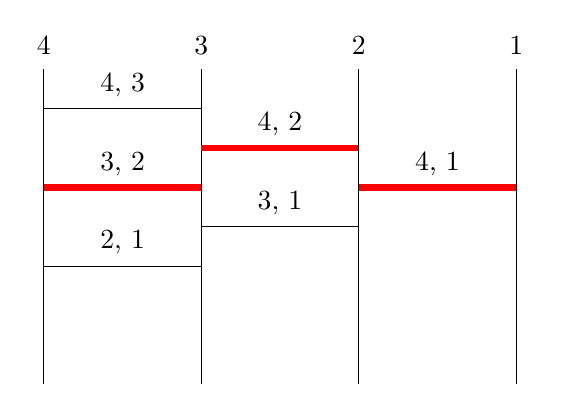
\begin{tikzpicture}
        \draw(0, 0) to (0, 4);
            \node at(0, 4.3){4};
             \draw(0, 3.5) to (2, 3.5);
                \node at(1, 3.8){4, 3};
            
            \draw[line width=0.8mm, red](0, 2.5) to (2, 2.5);
                \node at(1, 2.8){3, 2};

            \draw(0, 1.5) to (2, 1.5);
                \node at(1, 1.8){2, 1};
        \draw(2, 0) to (2, 4);
            \node at(2, 4.3){3};
                \draw[line width=.8mm, red](2, 3) to (4, 3);
                    \node at(3, 3.3){4, 2};
           
                \draw(2, 2) to (4, 2);
                    \node at(3, 2.3){3, 1};
        \draw(4, 0) to (4, 4);
             \node at(4, 4.3){2};
                \draw[line width=0.8mm, red](4, 2.5) to (6, 2.5);
                    \node at (5, 2.8){4, 1};
        \draw(6, 0) to (6, 4);
            \node at(6, 4.3){1};


    \end{tikzpicture}
    \end{center}
    \caption{The root ladder of $(4,3,2,1)$. Note that bar 4,2 is the parent of bar 3,2 and 4,1. Also note that 
    bar 3, 2 is the the left child of 4, 2 and 4, 1 is the right child.}
\end{figure}


